\documentclass[12pt, dvipsnames, svgnames, x11names,]{article}

\usepackage{xcolor}
% URLs and hyperlinks ---------------------------------------
\usepackage{hyperref}
\hypersetup{
	colorlinks=true,
	linkcolor=NavyBlue,
	filecolor=magenta,      
	urlcolor=blue,
}
\usepackage{xurl}
%---------------------------------------------------
\usepackage[inline]{enumitem}
\usepackage{graphicx}
\usepackage{multirow}
\usepackage{float}
\renewcommand{\arraystretch}{1.40}

% adjust a verrrrry big table -------------------------------
\usepackage{adjustbox}
% -----------------------------------------------------------

\usepackage{array}
% center the p columns and m --------------------------------------------------------------
\newcolumntype{P}[1]{>{\centering\arraybackslash}p{#1}}
\newcolumntype{M}[1]{>{\centering\arraybackslash}m{#1}}
% -------------------------------------------------------------------------------------------------------------

% price
\usepackage{marvosym}
% ----------

\usepackage{xepersian}
\settextfont{Arial}
\setdigitfont{Arial}

\begin{document}
	\begin{titlepage}
		\centering
		\vspace{1cm}
		{\Huge {\textbf{\lr{TF-IDF ranking}}}\par}
		\vspace{15mm}
		\vspace{16mm}
		
\includegraphics[width=12cm]{images/00.png} \par
		\vfill \par	\vfill
		\vspace{16mm}
		{\normalsize	سیدمحمدحسین هاشمی  4022363143 \par}
		\vspace{1cm}
		{\large فروردین ۱۴۰3\par}
	\end{titlepage}
	\tableofcontents
	\newpage
	
	
	\section{کتابخانه‌های مورد نیاز}

		\begin{center}
			{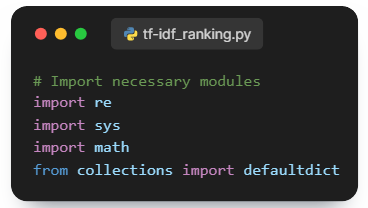
\includegraphics[width=6cm]{images/01.png}}
		\end{center}

		{\normalsize کتابخانه‌های مورد نیاز که در پروژه لود شده‌اند.}



	\section{کلاس \lr{Inverted Index}}

		\begin{center}
			{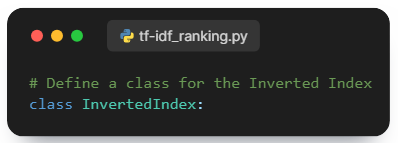
\includegraphics[width=7cm]{images/02.png}}
		\end{center}

		{\normalsize تمام کدهای مربوطه در این کلاس نوشته می‌شود}


	
	\section{متد \lr{--init--}}
		
		\begin{center}
			{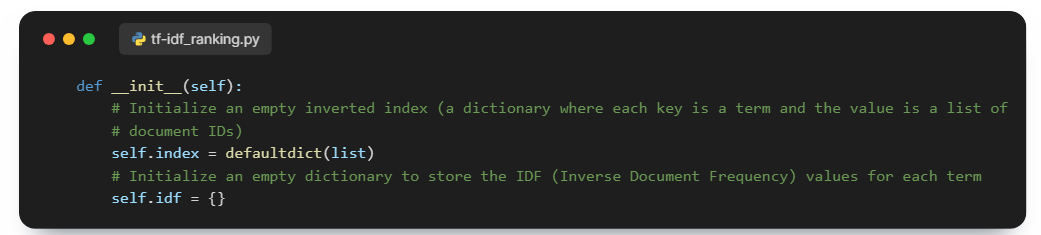
\includegraphics[width=11cm]{images/03.png}}
		\end{center}
		
		{\normalsize
			در اینجا یک کالکشن خالی برای ذخیره \lr{Inverted Index} و همچنین یک دیکشنری برای ذخیره \lr{idf} هر داکیومنت ایجاد می‌شود.
		} \par

	
	
	\section{متد \lr{add\_document}}
		
		\begin{center}
			{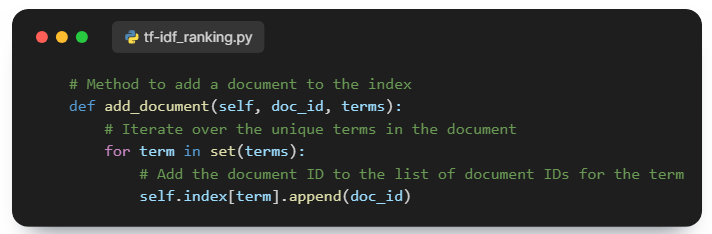
\includegraphics[width=8cm]{images/04.png}}
		\end{center}
		
		{\normalsize 
			در این متد عملیات اشتراک بین \lr{posting list}ها انجام می‌شود و نتیجه جست‌و‌جو برگشت داده می‌شود.
		}
		
	
	
		
	\section{متد \lr{rank\_document}}
	
		\begin{center}
			{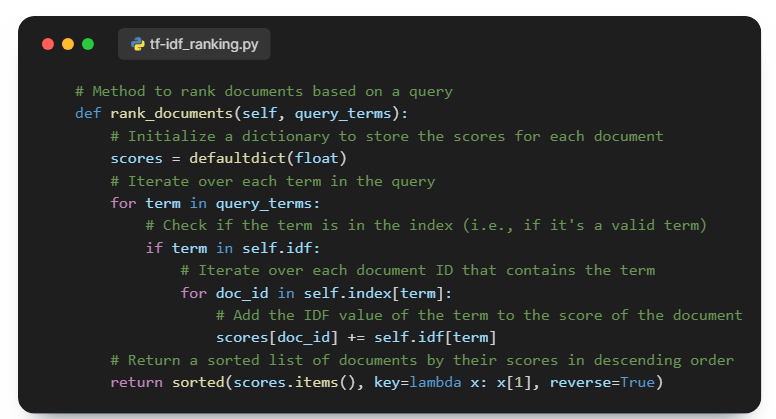
\includegraphics[width=10cm]{images/06.png}}
		\end{center}
	
		{\normalsize 
			در این تابع براساس ورودی (\lr{query\_terms}) با فرمول \lr{tf-idf} امتیازدهی انجام می‌شود و داکیومنت‌ها به‌ترتیب امتیاز برگشت‌داده می‌شوند.	
		}
		
		
			
	\section{استفاده}
	
		\begin{center}
			{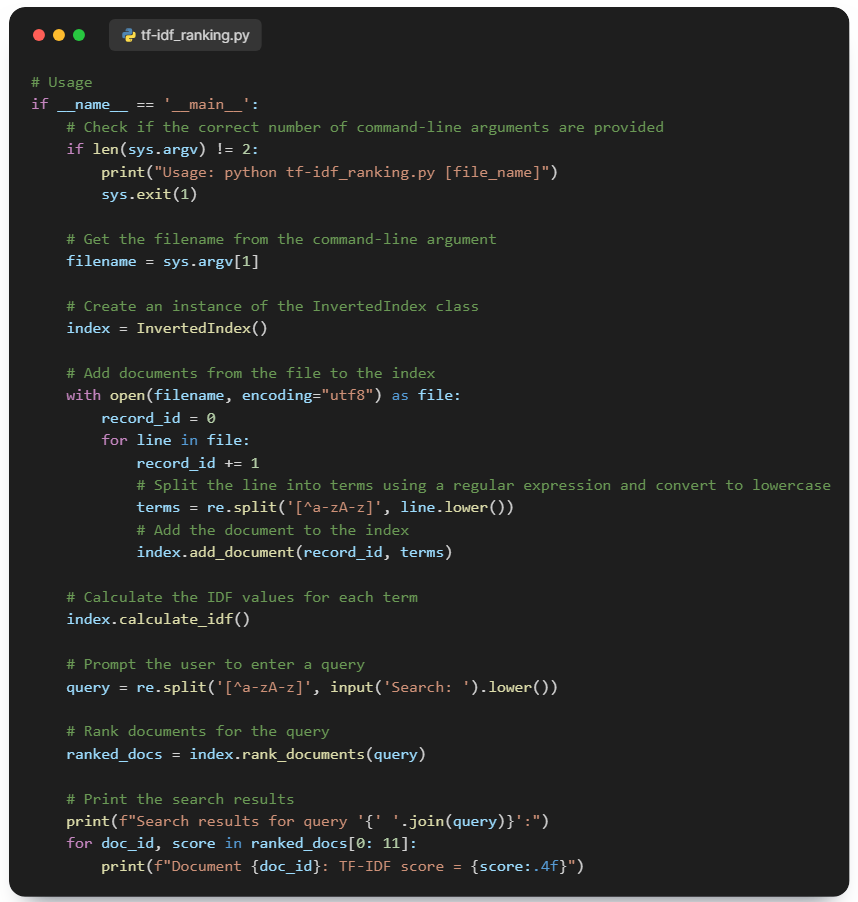
\includegraphics[width=10cm]{images/07.png}} \par
		\end{center}
	
		{\normalsize 
			برای استفاده از کلاس گفته شده این کد نوشته شده که بعد از فراخوانی کلاس ایجاد شده و پس از خواندن داکیومنت‌ها و ایجاد \lr{Inverted Index} در آن با استفاده از رنکینگ \lr{tf-idf} جست‌و‌جو انجام می‌شود و 10 نتیجه اول به همراه امتیاز خروجی داده می‌شود.
		}		
	
		{\normalsize برای مثال برای ورودی مانند تصویر زیر:}
	
		\begin{center}
			{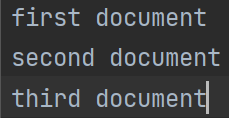
\includegraphics[width=6cm]{images/08.png}} \par
		\end{center}
	
		{\normalsize خروجی مانند تصویر زیر تولید می‌شود.}
	
		\begin{center}
			{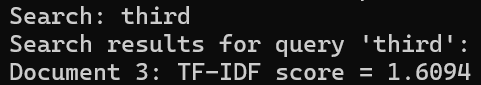
\includegraphics[width=6cm]{images/09.png}} \par
		\end{center}
	
	
	
\end{document}